Ввод и вывод данных, а также формирование массива результатов оформить как отдельные функции. Проверку существования результата произвести в главной программе. К элементам массива структур обращаться при помощи указателя. Для ввода данных и вывода результатов использовать функции fscanf, fgets. fputs и fprintf во второй программе. Написать программу, которая вводит в режиме запросов заданное число структур вида (1). После ввода массива структур программа ищет в нем все цвета самых дорогих автомобилей.
\begin{figure}[h]
    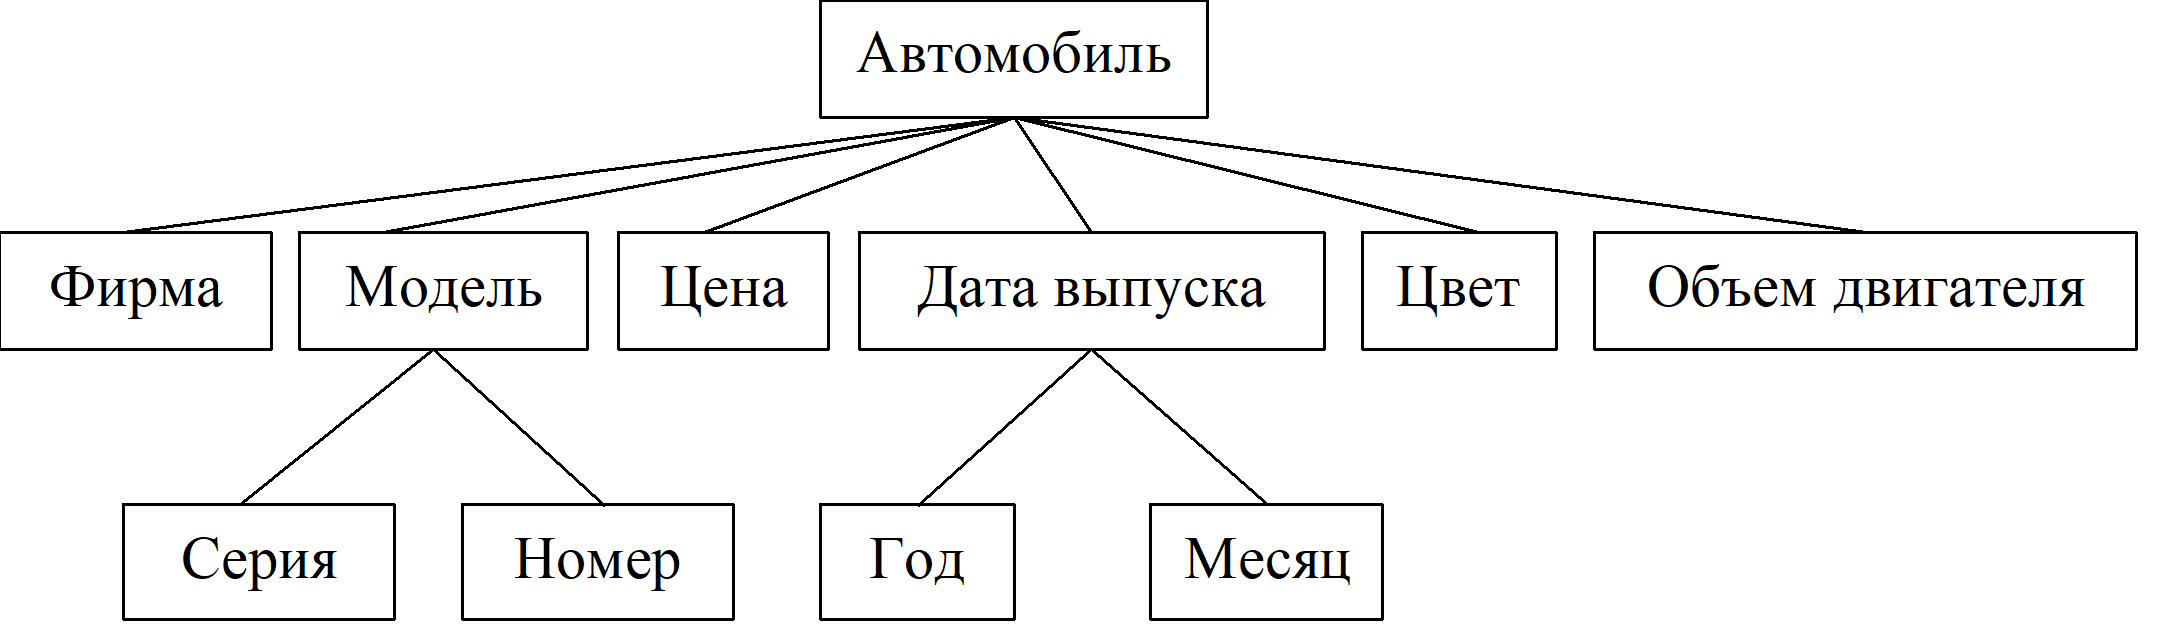
\includegraphics[scale=0.3]{zzz.png}
    \caption{}
\end{figure}
